% +------------------------------------------------------------------------+
% | Skin_surface_3/doc_tex/Skin_surface_3/SkinSurface3.tex
% +------------------------------------------------------------------------+
% | 2005 Nico Kruithof
% | Meshing the 3d Skin surface defined for a set of spheres.
% | 
\RCSdef{\skinSurfaceRev}{$Id$}
\RCSdefDate{\skinSurfaceDate}{$Date$}
% +------------------------------------------------------------------------+

\newcommand\ssWpoint[1]{{\bf #1}}
\newcommand\ssWeight[1]{w_{#1}}

\begin{ccTexOnly}
\begin{center}
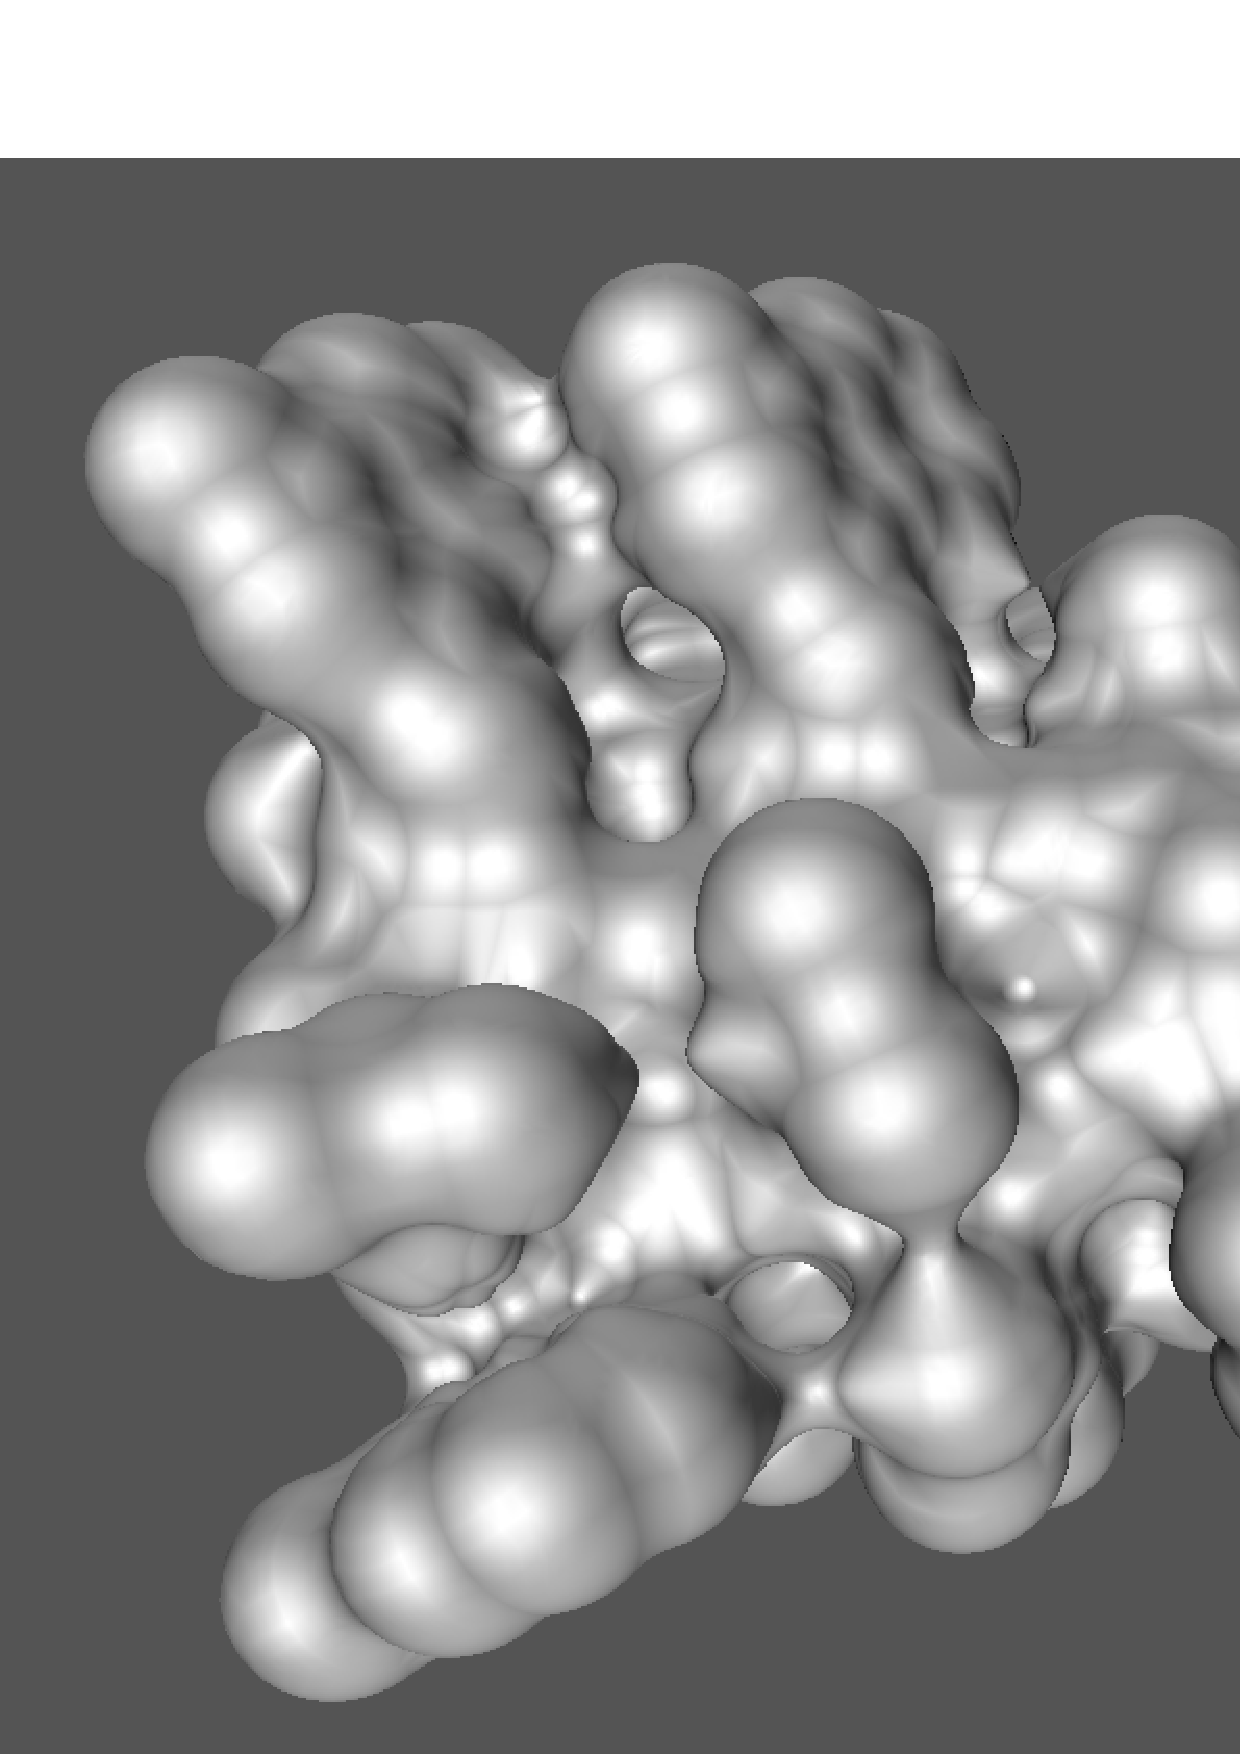
\includegraphics[width=.9\textwidth]{Skin_surface_3/molecule}
\end{center}
\end{ccTexOnly}
\begin{ccHtmlOnly}
  <center>
  <img border="0" src="./molecule.png" width="75%">
  </center>
\end{ccHtmlOnly}

% +------------------------------------------------------------------------+
\section{Introduction\label{sectionSkinSurfaceIntro}}

Skin surfaces, introduced by Edelsbrunner in \cite{cgal:e-dssd-99},
have a rich and simple combinatorial and geometric structure that
makes them suitable for modeling large molecules in biological
computing.  Meshing such surfaces is often required for further
processing of their geometry, like in numerical simulation and
visualization.

A skin surface is defined by a set of weighted points (input balls)
and a scalar called the shrink factor. If the shrink factor is equal
to one, the surface is just the boundary of the union of the input
balls.  For a shrink factor smaller than one, the skin surface becomes
tangent continuous, due to the appearance of patches of spheres and
hyperboloids connecting the balls.

This package constructs a mesh isotopic to the skin surface defined by
a set of balls and a shrink factor using the algorithm described in
\cite{cgal:kv-mssct-05}. %It also provides an interface to the surface
%mesher presented in Chapter~\ref{chapter_SurfaceMesher} by providing a
%model of the concept \ccc{Surface_3}.

An optimized algorithm is implemented for meshing the union of a set
of balls.

\section{Definition of a Skin Surface\label{sec:skindefinition}}

\begin{figure}
  \begin{ccTexOnly}
    \begin{center}
      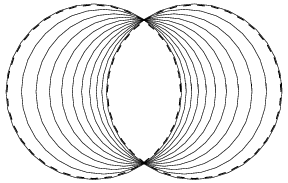
\includegraphics[width=.25\textwidth]{Skin_surface_3/convexTwoPoints}
      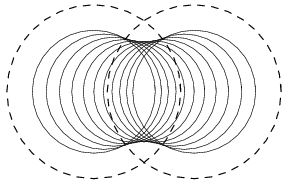
\includegraphics[width=.25\textwidth]{Skin_surface_3/skinTwoPoints}
    \end{center}
  \end{ccTexOnly}
  \begin{ccHtmlOnly}
    <center>
    <img border="0" src="./convexTwoPoints.png" align="center" alt="Convex combinations of two weighted points">
    <img border="0" src="./skinTwoPoints.png" align="center" alt="Skin
    curve of two weighted points">
    </center>
  \end{ccHtmlOnly}
  \caption{\label{fig:twoPoints} Left: Convex combinations of two
    weighted points (the two dashed circles). Right: The skin curve of
    the weighted points. The smaller circles form a subset of the
    weighted points whose boundary is the skin curve.}
\end{figure}

This section first briefly reviews skin surfaces. For a more thorough
introduction to skin surfaces, we refer to \cite{cgal:e-dssd-99} where
they were originally introduced.

A skin surface is defined in terms of a finite set of weighted points
$\ssWpoint{P}$ and a shrink factor $s$, with $0\leq s\leq 1$. A
weighted point $\ssWpoint{p}=({p},\ssWeight{p})\in \R^3\times\R$
corresponds to a ball with center ${p}$ and radius
$\sqrt{\ssWeight{p}}$. A weighted point with zero weight is called an
unweighted point. 

A pseudo distance between a weighted point $\ssWpoint{p} =
(p,\ssWeight{P})$ and an unweighted point $x$ is defined as
\[
\pi(\ssWpoint{p},x) = \dabs{p-x}^2 - \ssWeight{p},
\]
where $\dabs{p-x}$ is the Euclidean distance between $p$ and $x$.  The
ball corresponding to a weighted point $\ssWpoint{p}$ is the zero set
of $\pi(\ssWpoint{p},\cdot)$. Note that if $\ssWeight{p}<0$ the radius
of the ball is imaginary and the zero-set is empty.

We can take convex combinations of weighted points by taking convex
combinations of their distance functions.
%\[
%\pi(\gamma\; \ssWpoint{p} + (1-\gamma)\ssWpoint{q},x) =
%\gamma\; \pi(\ssWpoint{p},x) + (1-\gamma)\pi(\ssWpoint{q},x).
%\]
%hence the weighted point $\pi(\gamma\; \ssWpoint{p} +
%(1-\gamma)\ssWpoint{q},x)$ has center $\gamma\;p + (1-\gamma)q$ and
%weight $\gamma\;\ssWeight{p} + (1-\gamma)\ssWeight{q} +
%\gamma(1-\gamma)\dabs{p-q}$.
%
Figure~\ref{fig:twoPoints} (left) shows weighted points that
are obtained as convex combinations of the dashed circles. For further
reading on the space of circles and spheres we refer to
\cite{p-gcc-70}.

Starting from a weighted point $\ssWpoint{p}=({p},\ssWeight{P})$, the
shrunk weighted point $\ssWpoint{p}^s$ is obtained by taking a convex
combination with the unweighted point centered at $p$, formally
$\ssWpoint{p}^s = s \ssWpoint{p} + (1-s) \ssWpoint{p}'$, with
$\ssWpoint{p}'=(p,0)$. A simple calculation shows that,
$\ssWpoint{p}^s = ({p},s\cdot \ssWeight{p})$.  The set
$\ssWpoint{P}^s$ is the set obtained by shrinking every weighted point
of $\ssWpoint{P}$ by a factor $s$: $\ssWpoint{P}^s = \{\ssWpoint{p}^s
\mid \ssWpoint{p}\in \ssWpoint{P}\}$. The shrunk weighted points of
Figure~\ref{fig:twoPoints} (left) are shown in
Figure~\ref{fig:twoPoints} (right).

We now define the skin surface $\mbox{skn}^{s}(\ssWpoint{P})$
associated with a set of weighted points $\ssWpoint{P}$. Consider the
set of weighted points obtained by taking the convex hull of the input
weighted points. A calculation shows that every weighted point lies
within the union of the input balls. Next, we shrink each weighted
point in the convex hull with the shrink factor $s$. Hence, we
multiply the radius of the corresponding (real) input circles with a
factor $\sqrt{s}$. The skin surface is the boundary of the union of
this set of weighted points:
\begin{eqnarray}
  \label{eq:defskin}
  \mbox{skn}^{s}(\ssWpoint{P})
  &=& \partial\;{\bigcup\{\ssWpoint{p}^s\mid 
                   \ssWpoint{p}\in \mbox{conv} (\ssWpoint{P})\}}.
\end{eqnarray}
%
Here $\mbox{conv}(\ssWpoint{P}) \subset \R^3\times\R$ is the convex
hull of a set of weighted points $\ssWpoint{P}$, whereas $\partial$
denotes the boundary -- in $\R^3$ -- of the union of the corresponding
set of balls.

Recall that each weighted point in the convex hull of the input
weighted points is contained in the union of the input weighted
points. Hence, for a shrink factor equal to one, the skin surface is
the boundary of the union of the input weighted points.

By definition of a skin surface, the weights of the input balls (their
radius-squared) are shrunk with a factor of $s$ and the skin surface
wraps around the shrunk input balls. In order to make the skin surface
wrap around the (unshrunk) input balls, we can first increase the
weights of the input balls by multiplying them with a factor $1/s$ and
then compute the skin surface.

\section{The Interface}
\ccThree{void}{b}{}
\ccThreeToTwo

The interface to the skin surface package consists of one main
function, taking a set of weighted points and a shrink factor and
outputting the meshed surface. Further, it defines classes and
functions and classed used to perform the main steps of the algorithm.
There are two global classes \ccc{Skin_surface_3} and
\ccc{Union_of_balls_3} both of which are models of the concept
\ccc{SkinSurface_3} and there are two functions to extract a mesh of
the skin surface (union of balls) from the objects of the
aforementioned classes. A final function takes a mesh and the
\ccc{Skin_surface_3} (\ccc{Union_of_balls_3}) object it is constructed
from and refines the mesh. This section describes these classes and
functions in more detail.

The main function of the skin surface package takes an iterator range
of weighted points, a shrink factor and the number of subdivision
steps and outputs a mesh in a \ccc{CGAL::Polyhedron_3}:

\ccGlobalFunction{
  template <class WP_iterator, class Polyhedron_3> 
  void make_skin_surface_mesh_3(
  Polyhedron_3 &p,
  WP_iterator begin, WP_iterator end, 
  FT shrink_factor=.5,
  int nSubdiv=0,
  bool grow_balls = true);}

Where, \ccc{FT} is the number type used by the \ccc{Weighted_points}.

To obtain more control over the algorithm, the different steps can
also be performed separately. First, a \ccc{Skin_surface_3} object is
created from an iterator range of weighted points and a shrink factor.
Optional arguments are a boolean telling whether the input weighted
points should be grown in such a way that the skin surface wraps
around the input balls instead of the shrunk input balls.

\ccGlobalFunction{
  template <class SkinSurfaceTraits_3> 
  Skin_surface_3(
  WP_iterator begin, WP_iterator end, 
  FT shrink_factor,
  bool grow_balls = true);}

The template parameter should implement the \ccc{SkinSurfaceTraits_3}
concept. The type \ccc{WP_iterator}, is an iterator over weighted
points as defined by \ccc{SkinSurfaceTraits_3} and \ccc{FT} is the
number type used by the weighted points.


For a shrink factor equal to one the skin surface is the boundary of
the union of the input balls. In this case the algorithm used for
meshing the skin surface greatly simplifies. These optimizations are
implemented in the class \ccc{Union_of_balls_3}. The constructor for
the union of balls class is similar, except for the missing shrink
factor:

\ccGlobalFunction{
  template <class SkinSurfaceTraits_3> 
  Union_of_balls_3(
  WP_iterator begin, WP_iterator end, 
  bool grow_balls = true);}

With a model of the concept \ccc{SkinSurface_3} it is possible to
generate a coarse mesh isotopic to the skin surface. Using the
function \ccc{mesh_skin_surface_3} with signature:

\ccGlobalFunction{
  template <class SkinSurface_3, class Polyhedron>
  void mesh_skin_surface_3(const SkinSurface_3 &skin_surface, Polyhedron &p);}

The last function takes the (coarse) mesh and subdivides it in-situ by
applying a given number of 1-4 split operations (each triangle is
split into four sub-triangles) and moving the new vertices towards the
skin surface. If the number of iterations is not specified, one
subdivision step is done. The object of the \ccc{SkinSurface_3}
concept used to construct the coarse mesh is needed to move new points
on the skin surface.

\ccGlobalFunction{
  template <class SkinSurface_3, class Polyhedron >
  void subdivide_skin_surface_mesh_3 (
  const SkinSurface_3 &skinsurface,
  Polyhedron &p,
  int iterations=1);
}

%
%The class \ccc{Skin_surface_3} is both a model of the concept
%\ccc{SkinSurface_3} and the concept \ccc{Surface_3}.
%Therefore it can be used in the surface mesher described in
%Chapter~\ref{chapter_SurfaceMesher}.

\section{Timings}
The timings of the construction of the coarse mesh and the first
subdivision are given in seconds and were done on a Pentium 4, 3.5
GHz, with 1 Gb of memory.
\begin{center}
  \begin{tabular}{|l|c|c|c|}
    \hline
    Data set & Number of weighted points & Coarse mesh & first subdivision step\\
    \hline
    \hline
    Caffeine& 23 & 0.2 sec. & 0.05 sec.\\
    Gramicidin A& 318 & 5 sec. & 2 sec.\\
    \hline
  \end{tabular}
\end{center}

\section{Example Programs}
\subsection{Meshing a Skin Surface}
The following example shows the construction of a coarse mesh of the
skin surface using the function \ccc{make_skin_surface_mesh_3}. The
output is a \ccc{CGAL::Polyhedron}.
\ccIncludeExampleCode{Skin_surface_3/skin_surface_simple.cpp}

\subsection{Meshing and Subdividing a Skin Surface}
The following example shows the construction of mesh of the skin
surface by explicitly performing different steps of the algorithm. It
first constructs a \ccc{Skin_surface_3} object from an iterator range
of weighted points and a shrink factor. From this object, the coarse
mesh isotopic to the skin surface is extracted using the function
\ccc{CGAL::mesh_skin_surface_3}

Next, the coarse mesh is refined to obtain a better approximation. The
use of \ccc{CGAL::Skin_surface_polyhedral_items_3<Skin_surface_3>} in
the \ccc{CGAL::Polyhedron} is not necessary, but gives the subdivision
a significant speedup.
\ccIncludeExampleCode{Skin_surface_3/skin_surface_subdiv.cpp}



